\documentclass{report}[12pt]

\usepackage{geometry}[a4paper]
\usepackage{appendix}[toc]
\usepackage{inputenc}[uft8]
\usepackage{xeCJK}
\setCJKmainfont{Noto Serif CJK TC}
\usepackage{fontenc}[T1]
\usepackage{fontspec}
\setmainfont{Libertinus Serif}
\usepackage{bussproofs}
\usepackage{qtree}
\usepackage{amsmath}
\usepackage{amssymb}
\usepackage{amsthm}
\usepackage{tikz-cd}
\usepackage{tipa}
\usepackage{listings}
\usepackage[backend=biber, sorting=ynt, style=authoryear-icomp]{biblatex}
\addbibresource{hispania.bib}
\usepackage{xcolor}
\usepackage{epigraph}
\usepackage{bookmark}
\usepackage{tcolorbox}
\usepackage{colortbl}
\usepackage{mathtools}
\usepackage{stmaryrd}
\usepackage{footnote}
\makesavenoteenv{tabular}
\makesavenoteenv{table}
\usepackage{footmisc}[hang, flushmargin, bottom]
\usepackage{setspace} % alaways before hyperref, enabling correct footnote links
\usepackage{hyperref}[pdfencoding=auto, psdextra]
\hypersetup{
  colorlinks=true,
  linkcolor=violet,
  filecolor=magenta,
  citecolor=violet,
}
\usepackage{graphicx}
\graphicspath{{../pics/}}
\usepackage{unicode-math}
\setmathfont{Libertinus Math}
\usepackage{langsci-gb4e}
\usepackage{nameref}

\setlength\parindent{0pt}
\setlength\footnotemargin{0pt}
% \setcounter{secnumdepth}{3}

\title{El sueño de mi juventud: \\ Fonología automatizada}
\author{陳朝陽 \\ Chen Zhaoyang \\ \texttt{zc23@illinois.edu}}

\begin{document}

\maketitle

\pagebreak

\hspace{0pt}
\vfill

\begin{center}
  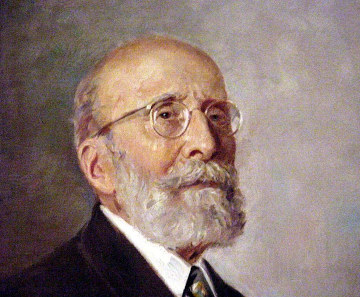
\includegraphics[scale=1.25]{pidal.jpg} \\
  \vspace{0.2cm}
  \Huge{Ramón Menédez Pidal \\ 1869 -- 1968}
\end{center}

\vfill  
\hspace{0pt}

\thispagestyle{empty}

\pagebreak

\hspace{0pt}
\vfill

\begin{minipage}{0.4\linewidth}
  \textbf{Invocation of Clio}\footcite{clio} \\

  I call to Clio, great of knowledge, \\
  daughter of Zeus and wise Mnemosyne, \\
  goddess who knows much of ancient days, \\
  of what has been, and thus of what may be. \\
  Great muse of history, you look to the past \\
  and understand its import and its might; \\
  you hold in your heart the lessons of time, \\
  the wisdom that has passed through the world. \\
  Through your power do we hear the words \\
  of those long gone, do we receive their counsel. \\
  Clio, chronicler of the good and the ill, \\
  I pray to you, goddess, I honor your gifts.
\end{minipage}
\begin{minipage}{0.6\linewidth}
  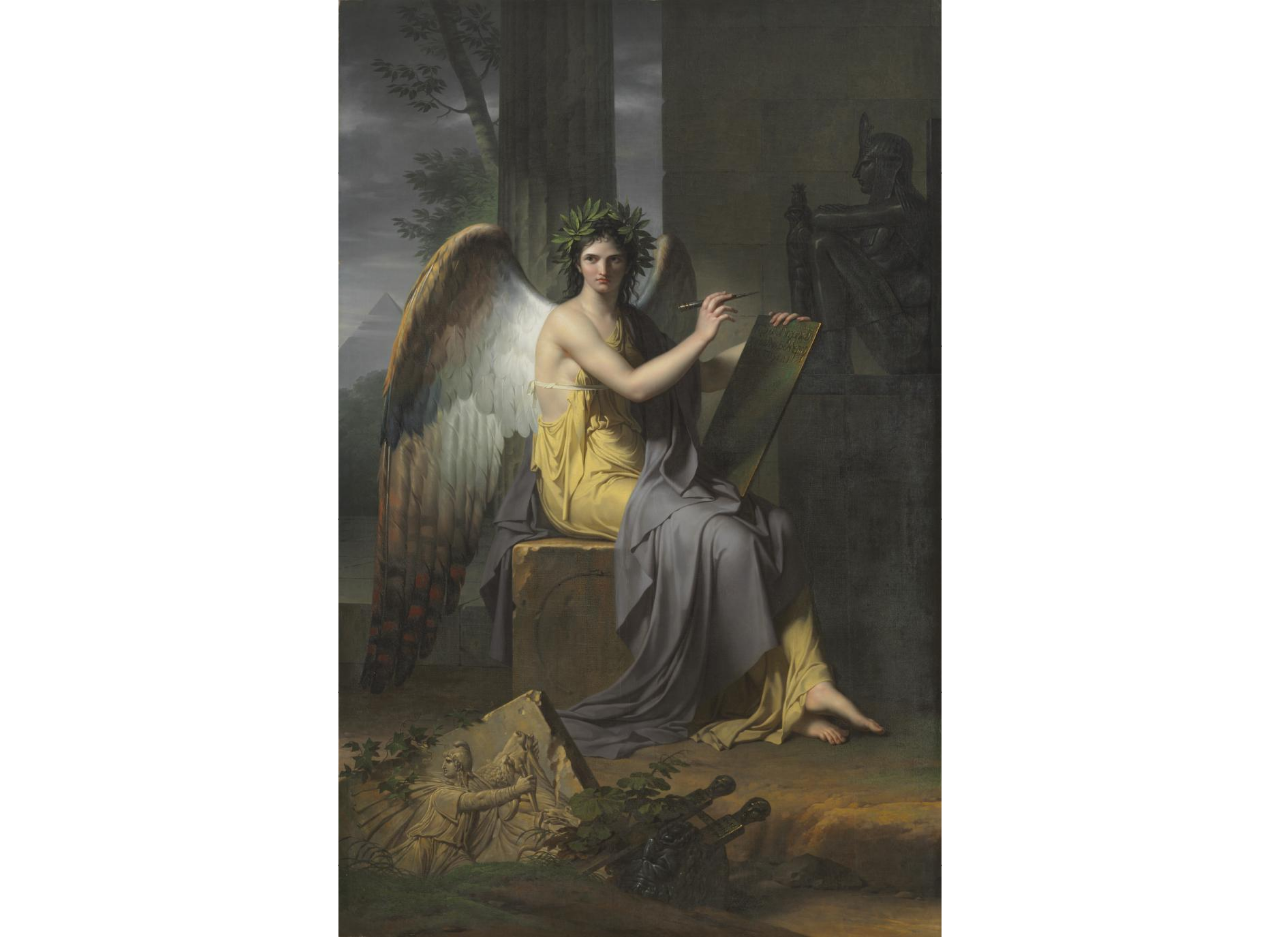
\includegraphics[scale=0.3]{clio.png}
\end{minipage}  

\vfill  
\hspace{0pt}

\thispagestyle{empty}

\pagebreak

\tableofcontents

\pagebreak

\chapter{Acknowledgements}

\epigraph{En adelanto van estos lugares: \\ ya tienen su diosa coronada.}{Leandro Díaz}

Finally, special thanks to Professor \textsc{Iosephus Ignatius Hualdus}, for his invaluable helps and advices in the writing of this paper. 

\begin{flushright}
Champaign, Illinois \\
Cambridge, England \\
C.Z.Y
\end{flushright}

\chapter{Introduction}

\epigraph{枯れた技術の水平思考\footnotemark}{横井軍平}
\footnotetext{\href{https://en.wikipedia.org/wiki/Gunpei_Yokoi\#Lateral_Thinking_with_Withered_Technology}{``Lateral Thinking of Withered Technology.''}}

\section{Seasoned Techniques}

This paper mainly uses \emph{seasoned} techniques in various fields -- meaning that the fundamental works this project builds on have been around for quite some time. 

\subsection{Rule-based Phonology}

The most fundamental technique used here, rule-based phonology, in itself a term coined by its aftecomers, has been around as its \emph{modern} form since at least late \texttt{'}\kern-1pt 60s. \\
At the beginning of the 20\textsuperscript{th} century, phonology, and historical linguisitcs, started to be formalized. After many years of formalization, around and after the publication of \emph{SPE}, the practice of phonology had long acquired a formal language, as we can see from the theoretic elegance and explanatory power of the phonology that \emph{SPE} pioneered.

\subsection{Romance Historical Linguistics}

The subject of study of this paper, Spanish, whose history belongs to the greater field of Romance historical linguistics, is one of the most ripened fruit of European historical linguistics since its birth. Countless literature are still being produced in this field. A couple of comprehensive monographs on the history of the Spanish language had been produced in English since the later half of the 20\textsuperscript{th} century e.g. \cite{penny_spanish} and \cite{lloyd_spanish}, among many others. This work is not possible without their scholarship.

\subsection{Typed Programming Languages}

The last piece of the \emph{puzle} [\texttt{'}puθ.le] is a \emph{typed programming language}. What does it have to do with typed programming languages? Well, the answer to this question is one of the two themes of this paper, other than giving a concise account of the phonological history of the Spanish language; I want to show that, phonology, which is a formal system, can be simulated by a computer. And this system can be quite naturally implemented in a so-called \emph{high-level programming language}.

\section{The Implementation of a Phonology}

In this paper we implement a kind of rule-based phonology that is capable of carrying out most of the historical sound changes from Latin to Modern Spanish. The underlying system and \emph{Phonology} (with a capital ``P'') is not language-specific. \\
We have observed that rule-based phonology primarily has two components: the \emph{statics}, in which rules are defined for constructing members of the surface representations in the phonology; and the \emph{dynamics}, in which rules are set for defining the transformations between the aforementioned surface representations. In the lingo of computation, phonology, just like computation, revolves around \emph{data} (segments, syllables etc.) and \emph{computation} (sound changes).

\part{Automated Phonology}
\addcontentsline{toc}{part}{Automated Phonology}

\chapter{The Little \emph{Metaphoner}}

Let us talk about the phonological notations and \emph{pseudocode} conventions used in this paper. The notations used in this paper are not to obfuscate but to illuminate our thoughts; this is the standard that we hold ourselves to. Though one may still ask: why invent yet another notation/language for phonology? I would answer by quoting \cite{abstracto} through \cite[p.~14]{squiggol}:
\begin{quote}
  Suppose a textbook has to be written for an advanced course in algorithmics [or phonology]. Which vehicle should be chosen to express the algorithms [or sound changes]? Clearly, one has the freedom to construct a new language, not only without the restaint of efficiency considerations, but without any considerations of implementability whatsoever.
\end{quote}
The pseudocode used in this paper (dubbed \emph{Metaphono} in homage to the work of \cite{hartman_phono}) is a \emph{functional} vernacular (inspired by the spirit, less the essence, of Bird-Meertens formalism\footcite{bird_moor, squiggol, bird_meertens_book}), which is quite close to the syntax and semantics of real world programming languages like Haskell \parencite{haskell2010} and Standard ML \parencite{def_sml}. Here I would quote \cite[p.~57]{abstracto} again to illustrate my understanding of \emph{Metaphono}:
\begin{quote}
  This pidgin ALGOL [in our case, the ML-Haskell creole\footnote{Maybe I should just call this language \emph{Vulgar ML}.}] is a language. It is not really a programming, nor a natural language, but it has characteristics from both. It is not steady, but evolving. How it will evolve we cannot know.
\end{quote}
In any regards, programming language theory is not the focus of this paper, whenever formalism becomes a burden in the clarification of our ideas, we take the liberty to explain them in a natural language. \\
The socratic style used in this chapter follows that of the book \emph{The Little LISPer} by \cite{lisper}.

\section{\emph{The Sound Patterns}}

\subsection*{\textsc{seg} $\vdash$ feat}

\begin{tcolorbox}
  \textcolor{violet}{What is [\textipa{T}]}? \quad [\textipa{T}] is a segment. \\
  \textcolor{violet}{What is \textsc{fricative}?} \quad It is a \emph{feature}. \\
  \textcolor{violet}{Is \textipa{T} a fricative?} \quad Yes, it is. \\
  \textcolor{violet}{\textipa{T} $\vdash$ fricative} \quad What does this mean? \\
  \textcolor{violet}{It means that [\textipa{T}] is a fricative.} \quad Is [\textipa{T}] also some other things? \\  
  \textcolor{violet}{Yes:}
  \begin{tcolorbox}
    \begin{align*}
    \text{\textipa{T}}\ & \vdash \text{non-sibilant fricative} \\
                      & \vdash \text{dental} \\
                      & \vdash \text{voiceless} 
    \end{align*}
  \end{tcolorbox}
  I feel like I have seen things of this sort before. \\
  \textcolor{violet}{The $\vdash$ or $\dashv$ symbol can just be read as ``is'' or ``exhibits the feature \dots''; this is in line with the \emph{SPE}\footcite{spe} style notation $\textbf{C}_{\text{[+feat]}}$.} \\ 
  Thank you, Noam and Morris. \\
\end{tcolorbox}

\subsection*{[feat$_1$ $\rightarrow$ feat$_2$] \textsc{seg}}

\begin{tcolorbox}
  \textcolor{violet}{What's the difference between [s] and [z]?} \quad [z] is voiced; while [s] is not. \\
  \textcolor{violet}{Do they differ in anything else?} \quad No. \\
  \textcolor{violet}{$[\text{voiceless} \rightarrow \text{voiced}]\ \text{s} \Rightarrow \text{z}$} \quad What does this mean? \\
  \textcolor{violet}{Change the \emph{feature} of \textsc{voicing} from \emph{voiceless} to \emph{voiced.}} \quad I see. \\  
\end{tcolorbox}

This notation has its roots in $\lambda-$calculi and other formal languages alike, this particular form is adopted from \cite{tpl}. The semantics of this notation is simple: rewrite \textbf{feat}$_1$ to \textbf{feat}$_2$ within \textsc{seg}.

\section{The Vernacular}

\subsection*{val : $\tau$}

\begin{tcolorbox}
  \textcolor{violet}{What is [\textipa{S}]?} \quad [\textipa{S}] is a consonant. \\
  \textcolor{violet}{Is [\textipa{S}] a vowel?} \quad No, it is not. \\
  \textcolor{violet}{\textipa{S} : Consonant} \quad What does this mean? \\
  \textcolor{violet}{It means that [\textipa{S}] is a consonant.} \quad What is a [a]? \\
  \textcolor{violet}{a : Vowel} \quad So [a] is a vowel. \\
\end{tcolorbox}

\subsection*{$\lambda$ : $\tau$ $\rightarrow$ $\tau$}

Functions are defined as such.
\begin{align*}
\text{\textcolor{magenta}{raise}} &\ :\ \text{Vowel} \rightarrow \text{Vowel} \\
\text{a} & \Rightarrow \text{e} \\
\end{align*}
Not so surprisingly, giving \textcolor{magenta}{raise} an [a] would yield an [e].
\[ \text{\textcolor{magenta}{raise}}\ (\text{a} : \text{Vowel}) \Rightarrow \text{e} : \text{Vowel} \]

\subsection*{$\lambda\ x \Rightarrow x$}

Consider this sound change for some hypothetical language that has \{s z n m \textipa{\r*n} \textipa{\r*m}\}.
\begin{align*}
  \text{\textcolor{magenta}{obstruentize}} &\ :\ \text{Consonant} \rightarrow \text{Consonant} \\
  \textbf{C} \vdash \text{fricative} & \Rightarrow [\text{fricative} \rightarrow \text{stop}]\ \textbf{C} \\
  \textbf{C} \vdash \text{nasal} & \Rightarrow \textbf{match}\ \text{\textcolor{magenta}{voice}}\ \textbf{C}
                                   \begin{cases}
                                     \text{voiced} & \Rightarrow [\text{nasal} \rightarrow \text{stop}]\ \textbf{C} \\
                                     \text{voiceless} & \Rightarrow [\text{nasal} \rightarrow \text{stop};\ \text{unaspirated} \rightarrow \text{aspirated}]\ \textbf{C} \\
                                   \end{cases}
\end{align*}

\begin{align*}
  \text{\textcolor{magenta}{obstruentize}}\ \text{s} & \Rightarrow \text{t} \\
  \text{\textcolor{magenta}{obstruentize}}\ \text{z} & \Rightarrow \text{d} \\
  \text{\textcolor{magenta}{obstruentize}}\ \text{n} & \Rightarrow \text{d} \\
  \text{\textcolor{magenta}{obstruentize}}\ \text{m} & \Rightarrow \text{b} \\
  \text{\textcolor{magenta}{obstruentize}}\ \text{\textipa{\r*n}} & \Rightarrow \text{\textipa{t\super h}} \\
  \text{\textcolor{magenta}{obstruentize}}\ \text{\textipa{\r*m}} & \Rightarrow \text{p\super h} \\
\end{align*}

\begin{align*}
  \lambda &\ :\ \tau \rightarrow \tau \\
  \text{pattern}_0 & \Rightarrow \text{exp}_0 \\
  \vdots & \\
  \text{pattern}_\omega & \Rightarrow \text{exp}_\omega \\
\end{align*}

\begin{align*}
  \textbf{match}\ \text{exp} & \begin{cases}
                                 \text{pattern}_0 & \Rightarrow \text{exp}_0 \\
                                                  & \vdots \\
                                 \text{pattern}_\omega & \Rightarrow \text{exp}_\omega \\
                               \end{cases}\\
\end{align*}

\subsection*{$\lambda : \tau \rightarrow \tau \rightarrow \tau$}

\subsection*{$(\lambda : (\tau \rightarrow \tau) \rightarrow \tau \rightarrow \tau)\ (\lambda' : \tau \rightarrow \tau)$}

\subsection*{Production Rules}

\subsection*{Common Types}

\subsection*{Hoare Logic}

\subsection*{Functor}

\chapter{In the Beginning was the \emph{Word}: \\ Segments, Syllables, and Lexemes}

\epigraph{En el principio existía la Palabra y la Palabra estaba con Dios, y la Palabra era Dios.}{Juan 1:1}

\section{Representation of Segments}

\subsection{Vocalic}

\begin{lstlisting}[basicstyle=\ttfamily, mathescape, escapeinside={(:}{:)}]
  vowel ::= height (:$\times$:) centrality (:$\times$:) duration

  height ::= low | low-mid | mid | high-mid | high

  centrality ::= front | central | back

  duration ::= short | long
\end{lstlisting}

\begin{tabular}{|c|c|c|c|}
  \hline
  & Front & Central & Back \\
  \hline
  High & i & & u \\
  \hline
  High-Mid & \textipa{I} & & \textipa{U} \\
  \hline
  Mid & e & & o \\
  \hline
  Low-Mid & \textipa{E} & & \textipa{O} \\
  \hline
  Low & & a & \\
  \hline
\end{tabular}

\subsection{Consonantal}

\begin{lstlisting}[basicstyle=\ttfamily, mathescape, escapeinside={(:}{:)}]
  consonant ::= manner (:$\times$:) place (:$\times$:) voice

  manner ::= nasal
           | stop
           | fricative
           | non-siblant fricative
           | affricate
           | approximant
           | tap
           | trill
           | lateral

  place ::= bilabial
          | labiodental
          | dental
          | alveolar
          | palatal
          | velar | labiovelar
          | glottal

  place ::= voiced | voiceless
\end{lstlisting}

\section{Representation of Syllables and Lexemes}

\subsection{Syllabic Structure}

\begin{lstlisting}[basicstyle=\ttfamily, mathescape, escapeinside={(:}{:)}]
  syllable ::= onset rhyme

  onset ::= zero-onset
          | monoonset consonant
          | dionset consonant(:$_1$:) consonant(:$_2$:)
          | trionset consonant(:$_1$:) consonant(:$_2$:) consonant(:$_3$:)
          
  rhyme ::= nucleus coda

  nucleus ::= zero-nucleus | monophthong vowel | diphthong vowel(:$_1$:) vowel(:$_2$:)

  coda ::= zero-coda
         | monocoda consonant
         | dicoda consonant(:$_1$:) consonant(:$_2$:)
\end{lstlisting}

\Tree [.$\sigma$ [.$\Omega$ [.π ] [.$\omega$ ] [.$\mu$ ] ] [.$\rho$ [\qroof{μν. | δφ.}.$\nu$ ] [.K [.$\kappa$ ] [.$\kappa'$ ] ] ] ]

Under this schema, the utterance-initial onset clusters would like this in Modern Spanish\footcite[p.~74]{hualde_sp}:
\begin{center}
\begin{tabular}{c|c}
  $\omega$ & $\mu$ \\
  \hline
  \begin{tabular}{c}
    p \textipa{B} t d k$^{\text{(w)}}$ g$^{\text{(w)}}$ \\
    f \textipa{T} s x \\
    \textipa{J} \\
    \textipa{\textteshlig} \\
    m n \textipa{\textltailn} \\
    l \textipa{L} \textipa{R} \\
  \end{tabular} & $\varnothing$ \\
  \hline
  \begin{tabular}{c}p b t d k g \\ f\end{tabular} & \textipa{R} \\
  \hline
  \begin{tabular}{c}p b (t) k g \\ f\end{tabular} & l \\
  \hline
\end{tabular}
\end{center}
And the utterance-final coda clusters\footcite[p.~75]{hualde_sp}:
\begin{center}
\begin{tabular}{c|c}
  $\kappa$ & $\kappa'$ \\
  \hline
  \begin{tabular}{c}
    p t d k \\
    f \textipa{T} s \\
    j \\
    n m \\
    l \textipa{R} \\
  \end{tabular}& $\varnothing$ \\
  \hline
  \begin{tabular}{c}
    p t k \\
    f \\
    n \\
    l \textipa{R} \\
  \end{tabular} & s \\
  \hline
  (n) & (\textipa{T}) \\
  \hline
\end{tabular}
\end{center}

\subsection{Syllable Weight and Stress}

Before we can discuss the stress pattern in Latin, it is necessary that we define a function to decide the weight of a syllable in Latin.
\begin{align*}
  \text{\textcolor{magenta}{weight}}\ & :\ \text{Syllable} \rightarrow \text{Weight} \\
  \sigma\ \vdash \Tree [.\text{$\rho$} [.\text{$\nu$} [.\textbf{V} ] ] [.K [.\text{$\varnothing$} ] ] ] & \Rightarrow \text{light} \\
  \sigma\ \vdash \Tree [.\text{$\rho$} [\qroof{\textbf{V:}\ | δφ.}.\text{$\nu$} ] [.K [.\text{$\varnothing$} ] ] ] & \Rightarrow \text{heavy} \\
  \sigma\ \vdash \Tree [.\text{$\rho$} [.\text{$\nu$} [.\textbf{V} ] ] [.K [.\text{$\kappa$} ] ] ] & \Rightarrow \text{heavy} \\
  \sigma\ \vdash \Tree [.\text{$\rho$} [.\text{$\nu$} [.\textbf{V} ]] [.K [.\text{$\kappa$} ] [.\text{$\kappa'$} ] ] ] & \Rightarrow \text{heavy} \\
\end{align*}
To have a concrete idea, see the following examples.
\begin{align*}
  \text{\textcolor{magenta}{weight}}\ \textsc{mi}_{\dashv\ \textsc{similis}} & \Rightarrow \text{light} \\
  \text{\textcolor{magenta}{weight}}\ \textsc{s\={o}}_{\dashv\ \textsc{pers\={o}na}} & \Rightarrow \text{heavy} \\
  \text{\textcolor{magenta}{weight}}\ \textsc{men}_{\dashv\ \textsc{fund\={a}mentum}} & \Rightarrow \text{heavy} \\
  \text{\textcolor{magenta}{weight}}\ \textsc{doc}_{\dashv\ \textsc{paradoxus}} & \Rightarrow \text{heavy} 
\end{align*}
After we are able to decide syllable weight, defining the Latin \textsc{penultimate} stress rule becomes natural.
\begin{align*}
  \text{\textcolor{magenta}{assign stress}} & :\ \text{List Syllable} \rightarrow \text{Lexeme} \\
  [\sigma] & \Rightarrow \begin{aligned}
                                                            & \textbf{let}\ \sigma' = [\text{unstressed} \rightarrow \text{stressed}] \ \sigma \\
                                                            & \textbf{in}\ \text{\textcolor{magenta}{mkLexeme}}\ [\sigma'] \\
                                                          \end{aligned} \\
  [\sigma_1 \dblcolon \sigma_2] & \Rightarrow \begin{aligned}
                                                            & \textbf{let}\ \sigma' = [\text{unstressed} \rightarrow \text{stressed}] \ \sigma_1 \\
                                                            & \textbf{in}\ \text{\textcolor{magenta}{mkLexeme}}\ [\sigma' \dblcolon \sigma_2] \\
                                                          \end{aligned} \\
  [\sigma^{*}]\ \texttt{++}\ [\sigma_1 \dblcolon \sigma_2 \dblcolon \sigma_3] & \Rightarrow \textbf{match}\ \text{\textcolor{magenta}{weight}}\ \sigma_2
                                                      \begin{cases}
                                                        \text{heavy} & \Rightarrow \begin{aligned}
                                                                                     & \textbf{let}\ \sigma' = [\text{unstressed} \rightarrow \text{stressed}]\ \sigma_2 \\
                                                                                     & \textbf{in}\ \text{\textcolor{magenta}{mkLexeme}}\ [\sigma^{*}]\ \texttt{++}\ [\sigma_1 \dblcolon \sigma' \dblcolon \sigma_3] \\
                                                                                   \end{aligned} \\
                                                        \text{light} & \Rightarrow \begin{aligned}
                                                                                     & \textbf{let}\ \sigma' = [\text{unstressed} \rightarrow \text{stressed}]\ \sigma_1 \\
                                                                                     & \textbf{in}\ \text{\textcolor{magenta}{mkLexeme}}\ [\sigma^{*}]\ \texttt{++}\ [\sigma' \dblcolon \sigma_2 \dblcolon \sigma_3] \\
                                                                                   \end{aligned} \\
                                                      \end{cases}
\end{align*}

\subsection{Syllabification}

\begin{align*}
  \text{\textcolor{magenta}{syllable empty?}} &\ :\ \text{Syllable} \rightarrow \text{Bool} \\
  \sigma \vdash \Tree [.\text{$\rho$} [.\text{$\nu$} [.\text{$\varnothing$} ] ] [.\text{K} ] ] & \Rightarrow \text{True} \\
  \_ & \Rightarrow \text{False} \\
\end{align*}

\chapter{Tilting against Windmills: \\ Sound Changes and Phonotactics}

\epigraph{星翳燈幻露泡夢電雲\footnotemark}{金剛經 \S32}
\footnotetext{\href{https://www2.hf.uio.no/polyglotta/index.php?page=record\&vid=1176\&mid=1993243}{A shooting star, a clouding of the sight, a lamp, an illusion, a drop of dew, a bubble, a dream, a lightning's flash, a thunder cloud.} Diamond Sutra \S32}

\section{Representation of Sound Changes}

\section{Rule Ordering}

\epigraph{Die ganzen Zahlen hat der liebe Gott gemachet, alles andere ist Menschenwerk}{Leopold Kronecker}

Recall that the natural numbers look like this: $\mathbb{N} \coloneq 0 \sqsubset 1 \sqsubset 2 \sqsubset 3 \sqsubset \dots \sqsubset \omega$.

\section{Representation of Phonotactics}

\part{A Phonological History of Spanish}

\chapter{Misc. Remarks and Comments}

\subsection*{Sources for Lat.-Rom.-Es. Gloss.}

The majority of the words in examples in this paper comes from \cite{romance_his}, \cite{lloyd_spanish}, and \cite{penny_spanish}. 

\pagebreak

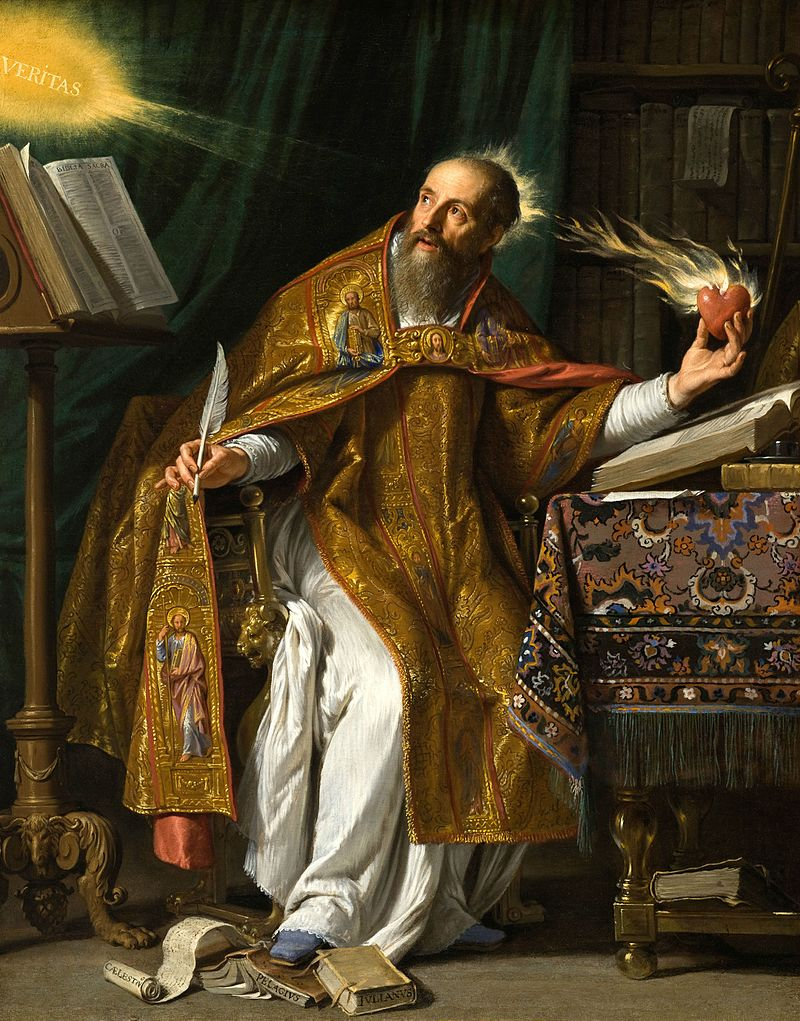
\includegraphics[scale=0.5]{augustine.jpg}

\thispagestyle{empty}

\pagebreak

\chapter{Proto-Romance}

\epigraph{\textsc{finis origine pendent}}{\textsc{marcvs manilivs}}

\emph{Proto-Romance}, among other terms like \emph{Vulgar Latin} and \emph{Popular Latin}, denotes a reconstructed language that evolved into the surviving Romance languages. 

\section{Phonemic Inventory}

\subsection{Vocalic}

\begin{tcolorbox}[hbox, title=Proto-Romance Monophthongs]
  \begin{tabular}{|c|c|c|c|}
    \hline
    & Front & Central & Back \\
    \hline
    High & i & & u \\
    \hline
    Mid & e & & o \\
    \hline
    Low-Mid & \textipa{E} & & \textipa{O} \\
    \hline
    Low & & a & \\
    \hline
  \end{tabular}
\end{tcolorbox}

\subsection{Consonantal}

\begin{tcolorbox}[title=Proto-Romance Consonants, hbox]
  \begin{tabular}{|c|c|c|c|c|c|c|c|}
    \hline
    & Bilabial & Labiodental & Dental & Alveolar & Palatal & Velar & Labiovelar \\
    \hline
    Nasal & m & & \multicolumn{2}{c|}{n} & \textipa{\textltailn} & & \\
    \hline
    Stop & p \quad b & & t \quad d & & & k \quad g & \textipa{k\super w} \quad \textipa{g\super w} \\
    \hline
    Fricative & \textipa{B} & f & & & \textipa{J} & & \\
    \hline
    \textquotedbl & & & & s \quad z & & & \\
    \hline
    Affricate & & & \textipa{\texttslig} \quad \textipa{\textdzlig} & & \textipa{\textteshlig} \quad \textipa{\textdyoghlig} & & \\
    \hline
    Trill & & & \multicolumn{2}{c|}{r} & & & \\
    \hline
    Lateral & & & \multicolumn{2}{c|}{l} & \textipa{L} & & \\
    \hline
  \end{tabular}
\end{tcolorbox}

\section{Sound Changes}

\subsection{Vocalism}

\subsubsection{Loss of Vowel Quantity}\label{sec:loss_of_quantity}

\begin{tcolorbox}
  \begin{tabular}{c c}
    \begin{tabular}{|c|c|c|c|c|c|c|}
      \hline
      & \multicolumn{2}{c|}{Front} & \multicolumn{2}{c|}{Cent.} & \multicolumn{2}{c|}{Back} \\
      \hline
      High & \cellcolor{gray} \textsc{\u{i}} & \textsc{\={i}} & & & \cellcolor{gray} \textsc{\u{u}} & \textsc{\={u}} \\
      \hline
      Mid & \cellcolor{gray} \textsc{\u{e}} & \textsc{\={e}} & & & \cellcolor{gray} \textsc{\u{o}} & \textsc{\={o}} \\
      \hline
      Low &  &  & \cellcolor{gray} \textsc{\u{a}} & \textsc{\={a}} & & \\
      \hline
    \end{tabular}
    \quad $\Rightarrow$ & 
                          \begin{tabular}{|c|c|c|c|}
                            \hline
                            & Front & Central & Back \\
                            \hline
                            High & i & & u \\
                            \hline
                            High-Mid & \cellcolor{magenta} \textipa{I} & & \cellcolor{magenta} \textipa{U} \\
                            \hline
                            Mid & e & & o \\
                            \hline
                            Low-Mid & \cellcolor{magenta} \textipa{E} & & \cellcolor{magenta} \textipa{O} \\
                            \hline
                            Low & & a & \\
                            \hline
                          \end{tabular}
  \end{tabular}
  \tcblower
  \begin{align*}\tag{Loss of Quantity}\label{eq:loss_of_quantity}
    \text{\textcolor{magenta}{loss of quantity}} &\ :\ \text{Vowel} \rightarrow \text{Vowel} \\
    \textbf{V} \vdash \text{long} & \Rightarrow [\text{long} \rightarrow \text{short}]\ \textbf{V} \\
    \textbf{V} \vdash \text{short} & \Rightarrow 
    \textbf{match}\ \textbf{V} \begin{cases}
                                \textbf{V} \vdash \text{low} & \Rightarrow \textbf{V} \\
                                \textbf{V} \vdash \text{mid} & \Rightarrow [\text{mid} \rightarrow \text{low-mid}]\ \textbf{V} \\
                                \textbf{V} \vdash \text{high} & \Rightarrow [\text{high} \rightarrow \text{high-mid}]\ \textbf{V} \\
                              \end{cases} \\
  \end{align*}
\end{tcolorbox}

Latin had a 5 vowel system with each vowel can be either long or short \parencites[p.~6]{romance_his}[p.~44]{penny_spanish}[p.~70]{lloyd_spanish}. Here are some minimal pairs showing the phonemic vowel length\footcite[p.~45]{penny_spanish}:
\begin{center}
  \begin{tabular}{c c c c}
    \textsc{h\={i}c} & `here' & \textsc{hic} & `this' \\
    \textsc{l\={i}ber} & `free' & \textsc{liber} & `book' \\
    \textsc{l\={e}vis} & `smooth' & \textsc{levis} & `light in weight' \\
    \textsc{v\={e}nit} & `he came' & \textsc{venit} & `he comes' \\
    \textsc{m\={a}lum} & `apple' & \textsc{malum} & `evil, misfortune' \\
    \textsc{\={o}s} & `mouth' & \textsc{os} & `bone' \\
    \textsc{p\={o}pulus} & `white poplar' & \textsc{populus} & `people' \\
  \end{tabular}
\end{center}
The distinction in vocalic quantity eventually collapsed \parencite[p.~112]{lloyd_spanish}:
\begin{quote}
  [I]n the fifth century St. Augustine remarked that in Africa people could not distinguish between long and short vowels. We may assume that he was referring to literary Latin since most of our evidence would indicate that spoken Latin had discarded quantity as a phonological feature long before then.
\end{quote}
The long vowels [i:], [u:], [e:], and [o:] did not change in quality, as it can be reflected in these Spanish reflexes\footcite[p.~12]{romance_his}:
\begin{center}
\begin{tabular}{c c}
  \textsc{latina} & Español \\
  \hline
  \textsc{v\textcolor{red}{\={i}}ta} & v\textcolor{magenta}{i}da \\
  \textsc{vic\textcolor{red}{\={i}}na} & vec\textcolor{magenta}{i}na \\
  \textsc{far\textcolor{red}{\={i}}na} & har\textcolor{magenta}{i}na \\
  \textsc{l\textcolor{red}{\={u}}na} & l\textcolor{magenta}{u}na \\
  \textsc{d\textcolor{red}{\={u}}ra} & d\textcolor{magenta}{u}ra \\
  \textsc{m\textcolor{red}{\={u}}ru} & m\textcolor{magenta}{u}ro \\
  \textsc{h\textcolor{red}{\={o}}ra} & h\textcolor{magenta}{o}ra \\
  \textsc{c\textcolor{red}{\={o}}rte} & c\textcolor{magenta}{o}rte \\
  \textsc{d\textcolor{red}{\={e}}bet} & d\textcolor{magenta}{e}be \\
  \textsc{t\textcolor{red}{\={e}}rnu} & t\textcolor{magenta}{e}rno \\
\end{tabular}
\end{center}
The long [a:] merges with the short [a]; while the short vowels [i], [u], [e] and [o] would experience lowering \parencite[p.~13]{romance_his}. As an interesting sidenote: in Sardinian, long and short vowels merge without changes in quality,yielding a five-vowel system \parencite[p.~112]{lloyd_spanish}.

\subsubsection{Great Merger}\label{sec:great_merger}

\begin{tcolorbox}
  \begin{tabular}{c c}
    \begin{tabular}{|c|c|c|c|}
      \hline
      & Front & Central & Back \\
      \hline
      High & i & & u \\
      \hline
      High-Mid & \cellcolor{gray} \textipa{I} & & \cellcolor{gray} \textipa{U} \\
      \hline
      Mid & e & & o \\
      \hline
      Low-Mid & \textipa{E} & & \textipa{O} \\
      \hline
      Low & & a & \\
      \hline
    \end{tabular}
    \quad $\Rightarrow$ &
                          \begin{tabular}{|c|c|c|c|}
                            \hline
                            & Front & Central & Back \\
                            \hline
                            High & i & & u \\
                            \hline
                            Mid & \cellcolor{magenta} e & & \cellcolor{magenta} o \\
                            \hline
                            Low-Mid & \textipa{E} & & \textipa{O} \\
                            \hline
                            Low & & a & \\
                            \hline
                          \end{tabular}
  \end{tabular}
  \tcblower
  \begin{align*}\tag{Great Merger}\label{eq:great_merger}
    \text{\textcolor{magenta}{great merger}} &\ :\ \text{Vowel} \rightarrow \text{Vowel} \\
    \text{\textipa{I}} & \Rightarrow \text{e} \\
    \text{\textipa{U}} & \Rightarrow \text{o} \\
  \end{align*}
\end{tcolorbox}

Later on, the vowel system of Romance languages continues to evolve, reducing the 9 vowel system shown above to a 7 vowel system \parencite[p.~13]{romance_his}: the high-mid vowels [\textipa{I}] and [\textipa{U}] would merge with their mid counterparts [e] and [u]\footcite[p.~14]{romance_his}:
\begin{center}
\begin{tabular}{c c c}
  \textsc{latina} & PrRom & Español \\
  \hline
  \textsc{g\textcolor{red}{u}la} & [\textipa{U}] & g\textcolor{magenta}{o}la \\
  \textsc{c\textcolor{red}{u}rrit} & [\textipa{U}] & c\textcolor{magenta}{o}rre \\
  \textsc{m\textcolor{red}{\u{u}}sca} & [\textipa{U}] & m\textcolor{magenta}{o}sca \\
  \textsc{b\textcolor{red}{i}b\textcolor{red}{i}t} & [\textipa{I}] & b\textcolor{magenta}{e}b\textcolor{magenta}{e} \\
  \textsc{l\textcolor{red}{i}ttera} & [\textipa{I}] & l\textcolor{magenta}{e}tra \\
  \textsc{v\textcolor{red}{\u{i}}ce} & [\textipa{I}] & v\textcolor{magenta}{e}z \\
\end{tabular}
\end{center}
For the low-mid vowels [\textipa{E}] and [\textipa{O}], both of them diphthongizes in either open or closed syllables in Spanish \parencite[p.~15-16]{romance_his}, later on in \nameref{sec:diphthongization_1} and \nameref{sec:diphthongization_2} we show the diphthongization of these vowels in details.

\subsubsection{Merger in Atonic Vowels}\label{sec:atonic_vowels}

\begin{tcolorbox}
  \begin{tabular}{c c}
    \begin{tabular}{|c|c|c|c|}
      \hline
      & Front & Central & Back \\
      \hline
      High & i & & u \\
      \hline
      Mid & e & & o \\
      \hline
      Low-Mid & \cellcolor{gray} \textipa{E} & & \cellcolor{gray} \textipa{O} \\
      \hline
      Low & & a & \\
      \hline
    \end{tabular} \quad $\Rightarrow$ & 
    \begin{tabular}{|c|c|c|c|}
      \hline
      & Front & Central & Back \\
      \hline
      High & i & & u \\
      \hline
      Mid & \cellcolor{magenta} e & & \cellcolor{magenta} o \\
      \hline
      Low & & a & \\
      \hline
    \end{tabular} \\
  \end{tabular} 
  \tcblower
  \begin{align*}\tag{Atonic Merger}\label{eq:atonic_merger}
    \text{\textcolor{magenta}{atonic merger}}\footnotemark &\ :\ \text{Vowel} \rightarrow \text{Vowel} \\
    \text{\textipa{E}} & \Rightarrow \text{e} \\
    \text{\textipa{O}} & \Rightarrow \text{o} \\
  \end{align*}
\end{tcolorbox}
\footnotetext{This function applies after \ref{eq:loss_of_quantity} and \ref{eq:great_merger}; but this is not \textbf{rule ordering}. The \emph{order of evaluation} is only important in this case because these vowel mergers are implemented in this particular way in for \emph{convenience} our system.}

So far in both \nameref{sec:loss_of_quantity} and \nameref{sec:great_merger} we mainly discussed the outcomes of \textbf{stressed} (\emph{tonic}) Latin-Romance vowels. The atonic vowels showed greater degrees of reduction than their tonic counterparts \parencite[p.~113]{lloyd_spanish}:
\begin{quote}
  The result [of the vowel system reduction in atonic vowels] was the coalescence of these [high and mid] vowels into two phonemes only: /i, e:, e/ > /e/, and /u, o:, o/ > /o/. Thus for vowels in these [unstressed] syllables a five vowel system was established[.] 
\end{quote}
Some examples for the outcomes of atonic vowels\footcite[p.~113]{lloyd_spanish}:
\begin{center}
  \begin{tabular}{c c}
    \textsc{lat.} & Es. \\
    \hline
    \textsc{h\={i}bern\textcolor{red}{u}} & iviern\textcolor{magenta}{o} \\
    \textsc{c\textcolor{red}{i}rc\={a}re} & c\textcolor{magenta}{e}rcar \\
    \textsc{v\={e}n\={a}t\textcolor{red}{u}} & venad\textcolor{magenta}{o} \\
  \end{tabular}
\end{center}

\subsubsection{Monophthongization}

\begin{tcolorbox}
  \begin{align*}
  \textsc{oe} & \Rightarrow \text{e} \\
  \textsc{au} & \Rightarrow \text{o}\ |\ \text{a} \\
  \textsc{ae} & \Rightarrow \text{\textipa{E}}\ |\ \text{e} \\
  \end{align*}
  \tcblower
  \begin{align*}\tag{Monophthongization}\label{eq:monophthongization}
    \text{\textcolor{magenta}{monophthongization}} &\ :\ \text{Vowel} \rightarrow \text{Vowel} \\
    \textsc{oe} & \Rightarrow \text{e} \\
    \textsc{au} & \Rightarrow \text{o}\ |\ \text{a}\footnotemark \\
    \textsc{ae} & \Rightarrow \text{\textipa{E}}\ |\ \text{e}\footnotemark \\
  \end{align*}
\end{tcolorbox}
\addtocounter{footnote}{-2}
\stepcounter{footnote}\footnotetext{\textsc{au} monophthongizes to [a] only when followed by a labialized velar e.g. \textsc{augusto} $\rightarrow$ \textsc{agusto} $\rightarrow$ Es. \emph{agosto}, \textsc{auscult\={a}re} $\rightarrow$ \textsc{ascult\={a}re} $\rightarrow$ OSp. \emph{ascuchar}, and \textsc{augurium} $\rightarrow$ \textsc{agurium} $\rightarrow$ Es. \emph{ag\"{u}ero} \parencite[p.~107]{lloyd_spanish}.}
\stepcounter{footnote}\footnotetext{\textsc{ae} giving [e:] is sporadic; sporadic changes like this in practice are implemented as another function (sound change); for simplicity's sake we list them like as if they are the same function.}

There were 3 diphthongs in Classical Latin that underwent monophthongization in its evolution to Popular Latin/Proto-Romance: \textsc{ae}, \textsc{oe}, and \textsc{au}. Although there were other diphthongs inherited from Indo-European (\textsc{ei} and \textsc{ov}) that had been merged with long vowels in the Old Latin period \parencite[p.~18]{companion_to_latin}:
\begin{quote}
  [F]rom the mid-second century \textsc{bce} the digraphs \textsc{ei} and \textsc{ov}, which earlier spelled inherited diphthongs, spelled the long vowels /iː/ and /uː/ respectively, regardless of their etymological source, e.g. \textsc{[v]eivam} /wiːwam/ ``living'' (\emph{CIL} I\textsuperscript{2}.1837), \textsc{covravervnt} /kuːraːweːrʊnt/ ``oversaw'' (\emph{CIL} I\textsuperscript{2}.1806).
\end{quote}
Here we focus on the 3 diphthongs that survived into Classical Latin. \\
The diphthong \textsc{ae} mainly reflects a short [\textipa{E}] \footcite[p.~105]{lloyd_spanish}:
\begin{center}
\begin{tabular}{c c}
  \textsc{lat.} & Es. \\
  \hline
  \textsc{caecu} & ciego \\
  \textsc{caelu} & cielo \\
  \textsc{quaero} & quiero \\
\end{tabular}
\end{center}
In some cases it would give a long [e:]\footcite[p.~105]{lloyd_spanish}:
\begin{center}
\begin{tabular}{c c}
  \textsc{lat.} & Es. \\
  \hline
  \textsc{caespite} & c\'{e}sped \\
  \textsc{faece} & hez \\
  \textsc{faenu} & heno \\
  \textsc{praeda} & prea \\
  \textsc{saepe} & sebe \\
  \textsc{saeptu} & seto \\
  \textsc{saeta} & seda \\
  \textsc{taeda} & tea \\
\end{tabular}
\end{center}
The diphthong \textsc{oe} would evolve into a long [e:]\footcite[p.~106]{lloyd_spanish} e.g. \textsc{foedus} $\rightarrow$ Es. feo\footcite[p.~23]{romance_his}:
\begin{center}
  \begin{tabular}{c c}
    \textsc{phoebus} & \textsc{phebus} \\
    \textsc{coena} & \textsc{c\={e}na} \\
    \textsc{poena} & \textsc{pena} \\ 
  \end{tabular}
\end{center}
And \textsc{au} gives a long vowel [o:]\footcite[p.~24]{romance_his}:
\begin{center}
\begin{tabular}{c c}
  \textsc{lat.} & Es. \\
  \hline
  \textsc{\textcolor{red}{au}ru} & \textcolor{magenta}{o}ro \\
  \textsc{thes\textcolor{red}{au}ru} & tes\textcolor{magenta}{o}ro \\
  \textsc{p\textcolor{red}{au}peru} & p\textcolor{magenta}{o}bre \\
  \textsc{p\textcolor{red}{au}cu} & p\textcolor{magenta}{o}co \\
\end{tabular}
\end{center}

\subsubsection{Loss of Hiatus}

\begin{tcolorbox}

\end{tcolorbox}

\begin{tabular}{c c}
  \textsc{lat.} & Es. \\
  \hline
  \textsc{qu\textcolor{red}{i\={e}}tu} & qu\textcolor{magenta}{e}do \\
  \textsc{par\textcolor{red}{i\u{e}}te} & par\textcolor{magenta}{e}d \\
\end{tabular}

\subsubsection{Syncope}

\begin{tcolorbox}
   \[ \textbf{C}\textbf{V}.\textbf{C} \Rightarrow \textbf{C}\textbf{C} \]
\end{tcolorbox}

``There was extensive syncope of atonic vowels in words having four or more syllables in prehistoric Latin, and this process continued throughout the historical period'' \parencite[p.~113]{lloyd_spanish}. \\
Here are some examples of syncope that were attested in Popular Latin\footcites[p.~28-29]{romance_his}[p.~114]{lloyd_spanish}:
\begin{center}
\begin{tabular}{c c}
  \textsc{lat.} & Pop. Lat. \\
  \hline
  \textsc{oc\textcolor{red}{u}lu} & \textsc{oclu} \\
  \textsc{auric\textcolor{red}{u}la} & \textsc{oricla} \\
  \textsc{cal\textcolor{red}{i}du} & \textsc{caldu} \\
  \textsc{ang\textcolor{red}{u}lus} & \textsc{anglus} \\
  \textsc{spec\textcolor{red}{u}lum} & \textsc{speclum} \\
  \textsc{vet\textcolor{red}{u}lus} & \textsc{veclus}\footnote{This is one of the words in which \textsc{-tl-} $\rightarrow$ \textsc{-cl-} \parencite[p.~68]{romance_his}.} \\
  \textsc{vir\textcolor{red}{i}dis} & \textsc{virdis} \\
\end{tabular}
\end{center}
And some that are reflected in Spanish\footcite[p.~29]{romance_his}:
\begin{center}
\begin{tabular}{c c}
  \textsc{lat.} & Es. \\
  \hline
  \textsc{lep\textcolor{red}{o}re} & liebre \\
  \textsc{i(n)s\textcolor{red}{u}la} & isla \\
  \textsc{vir\textcolor{red}{i}de} & verde \\
\end{tabular}
\end{center}
``The factor that seems to have had the greatest importance [in the application of syncope] was whether the consonants which came into contact after syncope formed normally occurring [consonant] groups in Latin'' \parencite[p.~114]{lloyd_spanish}. Here are more examples of syncopes and their contexts\footcite[p.~114]{lloyd_spanish}:
\begin{enumerate}
  \item \textbf{posttonic} \\
  \textsc{positus} $\rightarrow$ \textsc{postus} $\rightarrow$ Es. \emph{puesto} \\
  \textsc{suspendere} $\rightarrow$ \textsc{suspendre} \\
  \textsc{tabula} $\rightarrow$ \textsc{tabla}
  \item \textbf{pretonic} \\
  \textsc{maled\={i}x\={i}} $\rightarrow$ \textsc{maldixi} $\rightarrow$ Es. \emph{maldije}
\end{enumerate}
Occationally the syncopated and unsyncopated forms coexist in Spanish, usually the unsyncopated form being a \emph{cultismo} e.g. parab\textcolor{red}{o}la v. parabla. \\

\subsubsection{Apocope}

\begin{tcolorbox}

\end{tcolorbox}

\subsubsection{Metaphony}

\begin{tcolorbox}

\end{tcolorbox}

\subsection{Consonantism}

\begin{tcolorbox}[hbox, title=Latin Consonants]
  \begin{tabular}{|c|c|c|c|c|c|c|c|c|}
    \hline
    & Bilabial & Labiodental & Dental & Alveolar & Palatal & Velar & Labiovelar & Glottal \\
    \hline
    Nasal & m & & \multicolumn{2}{c|}{n} & & & & \\
    \hline
    Stop & p \quad b & & t \quad d & & & k \quad g & \textipa{k\super w} \textipa{g\super w} & \\
    \hline
    Fricative & & f & & & & & & \cellcolor{gray} h \\
    \hline
    \textquotedbl & & & & s \quad z & & & & \\
    \hline
    Approximant & & & & & \cellcolor{gray} j & & \cellcolor{gray} w & \\
    \hline
    Trill & & & \multicolumn{2}{c|}{r} & & & & \\
    \hline
    Lateral & & & \multicolumn{2}{c|}{l} & & & & \\
    \hline
  \end{tabular}
\end{tcolorbox}

\subsubsection{Prothesis}

\begin{tcolorbox}
  \[ \#\ \text{s} \Rightarrow \#\ \text{is} \]
\end{tcolorbox}

This phenomenon is attested in the Visigothic documents \parencite[p.~159]{latin_palaeography}:
\begin{quote}
  [T]he addition of \emph{i} at the beginning of a word that starts with an \emph{s} followed by another consonant (\emph{iscriptura}), or its suppression by hypercorrection (\emph{sta} for \emph{ista}).
\end{quote}

\begin{tabular}{c c}
  \textsc{lat.} & Es. \\
  \hline
  \textsc{\textcolor{red}{sp}onsa} & \textcolor{magenta}{esp}osa \\
  \textsc{\textcolor{red}{sp}ata} & \textcolor{magenta}{esp}ada \\
  \textsc{\textcolor{red}{st}udiu} & \textcolor{magenta}{est}udio \\
  \textsc{\textcolor{red}{sp}ongia} & \textcolor{magenta}{esp}onja \\
  \textsc{\textcolor{red}{sc}utu} & \textcolor{magenta}{esc}udo \\
\end{tabular}

\subsubsection*{Betacism I}

\begin{tcolorbox}
  \begin{align*}
    \text{w} & \Rightarrow \text{\textipa{B}} \\
    \text{b} & \Rightarrow \text{\textipa{B}} \\
  \end{align*}
\end{tcolorbox}

Visigothic spelling exhibits the ``[c]onfusion of \emph{u} and \emph{b} (\emph{haueo} for \emph{habeo}) or vice versa (\emph{pabor} for \emph{pauor})'' \parencite[p.~159]{latin_palaeography}.

\paragraph{Forition of [w] in Germanic Loanwords}

\begin{center}
\begin{tabular}{c c}
  Gm. & Es. \\  
  \hline
  \textcolor{red}{w}isa & \textcolor{magenta}{gu}isa \\
  \textcolor{red}{w}erra & \textcolor{magenta}{gu}erra \\
  \textcolor{red}{w}arten & \textcolor{magenta}{gu}ardar \\
  \textcolor{red}{w}ant & \textcolor{magenta}{gu}ante \\  
\end{tabular}
\end{center}

(PrBsq. *euscala $\rightarrow$) \textsc{lat.} \textsc{vasconem} $\rightarrow$ Es. Gasc\'{o}n

\subsubsection*{Yod Fortition}

\begin{tcolorbox}
  \begin{align*}
    \text{j-} \Rightarrow \text{\textipa{\textbardotlessj}} & \Rightarrow \text{\textipa{\textdyoghlig}} \\
    \text{-j-} \Rightarrow \text{\textipa{J}} & \Rightarrow \text{\textipa{\textipa{\textdyoghlig}}} \\
  \end{align*}
\end{tcolorbox}

\begin{tabular}{c c}
  \textsc{lat.} & Es. \\
  \hline
  \textsc{\textcolor{red}{i}ocu} & \textcolor{magenta}{j}uego \quad [x] \\
  \textsc{\textcolor{red}{i}vis} & \textcolor{magenta}{j}ueves \quad [x] \\
  \textsc{\textcolor{red}{i}uvene} & \textcolor{magenta}{j}oven \quad [x] \\
  \textsc{\textcolor{red}{i}udice} & \textcolor{magenta}{j}uez \quad [x] \\
\end{tabular}

\begin{tabular}{c c}
  \textsc{lat.} & Es. \\
  \hline
  \textsc{ma\textcolor{red}{i}us} & ma\textcolor{magenta}{y}o \\
  \textsc{ma\textcolor{red}{i}ore} & ma\textcolor{magenta}{y}or \\
  \textsc{cu\textcolor{red}{i}us} & cu\textcolor{magenta}{y}o \\
\end{tabular}

\begin{tabular}{c c}
  \textsc{lat.} & Es. \\
  \hline
  \textsc{\textcolor{red}{i}acet} & \textcolor{magenta}{y}ace \\
  \textsc{\textcolor{red}{i}am} & \textcolor{magenta}{y}a \\
\end{tabular}

Visigothic document witnesses ``[t]he use of \emph{g} instead of \emph{j} [\dots] (\emph{magor}) or \emph{i} instead of \emph{g} (\emph{ienitor})'', cf. \textsc{maior}, \textsc{genitor} \parencite[p.~159]{latin_palaeography}.

\subsubsection*{Deaspiration}

\begin{tcolorbox}
  \[ \text{h} \Rightarrow \varnothing \]
\end{tcolorbox}

We have evidence that initial /h/ already weakens in Latin: ``[i]n metrical texts final vowels are elided before words beginning with /h\textbf{V}/, exactly as before initial /\textbf{V}/.'' \parencite[p.~87]{companion_to_latin} \\
An orthographic evidence for this sound change was the fact that the letter <h> sometime was used to indicate hiatus between vowels in inscriptions \parencite[p.~18]{companion_to_latin}: \textsc{ahenvm}\footnote{cf. \textsc{a\={e}num}} [aeːnʊm] (\emph{CIL} I\textsuperscript{2}.581), \textsc{ahena}\footnote{cf. \textsc{a\={e}na}} (\emph{CIL} I\textsuperscript{2}.2093).

\begin{tabular}{c c}
  \textsc{lat.} & Es. \\
  \hline
  \textsc{hispalis} & Sevilla
\end{tabular}

\subsubsection*{Elision of Intervocalic [g]}

\begin{tcolorbox}
  \[ \textbf{V}.\text{g}\textbf{V} \Rightarrow \textbf{V}\textbf{V} \]
\end{tcolorbox}

\begin{tabular}{c c}
  \textsc{lat.} & Es. \\
  \hline
  \textsc{di\textcolor{red}{g}itu} & dedo \\
  \textsc{iam ma\textcolor{red}{g}is} & jamás \\
  \textsc{ma\textcolor{red}{g}istru} & maestro \\
  \textsc{sa\textcolor{red}{g}itta} & saeta \\
  \textsc{pa\textcolor{red}{g}ense} & país \\
  \textsc{c\={o}\textcolor{red}{g}it\={a}re} & cuidar \\
\end{tabular}

\subsubsection*{Elision of Coda [m]}

\begin{tcolorbox}
  \[ \text{m}\ \# \Rightarrow \varnothing\ \# \]
\end{tcolorbox}

The traces of this sound change go back to Old Latin (\emph{CIL} I\textsuperscript{2}.9) \parencite[p.~17]{companion_to_latin}: \\
\begin{tabular}{c c}
  Old Lat. & Class. Lat. \\
  \hline
  \textsc{oino} & \textsc{unum} \\
  \textsc{dvonoro} & \textsc{bonorum} \\
  \textsc{optumo} & \textsc{optimum} \\
  \textsc{viro} & \textsc{uirorum} \\
  \textsc{scipione} & \textsc{scipionem} \\
\end{tabular} \\
Also, ``[i]n metrical texts, where the the final syllables of words ending in /\textbf{V}/ $+$ <\textsc{m}> are treated in the same way as those in final /\textbf{V}/, being elided before a following initial /\textbf{V}/.'' \parencite[p.~87]{companion_to_latin}

\subsubsection*{Nasal Spirant Law}

\begin{tcolorbox}
  \[ \text{n.s} \Rightarrow \text{s} \]
\end{tcolorbox}

Old Latin inscriptions reflect this change \parencite[p.~17]{companion_to_latin}: \textsc{cosol} v. Class. Lat. \textsc{consul}, \textsc{cesor} v. Class. Lat. \textsc{censor} (\emph{CIL} I\textsuperscript{2}.8).

\subsubsection*{New Clusters from Syncope}

\paragraph*{Nasal Liquid Cluster from Syncope}

\begin{center}
\begin{tabular}{c c}
  \textsc{lat.} & Es. \\
  \hline
  \textsc{te\textcolor{red}{ner}u} & tie\textcolor{magenta}{rn}o \\
  \textsc{ge\textcolor{red}{ner}u} & ye\textcolor{magenta}{rn}o \\
  \textsc{tre\textcolor{red}{mul}at} & tie\textcolor{magenta}{mbl}a \\
\end{tabular}
\end{center}

\paragraph*{Nasal Nasal Cluster from Syncope}

\subsubsection*{Palatalization and Affrication of Dentals}

\begin{tcolorbox}
  \begin{align*}
    \text{ti} & \Rightarrow \text{\textipa{\texttslig}} \\
    \text{di} & \Rightarrow \text{\textipa{\textdyoghlig}} \\
  \end{align*}
\end{tcolorbox}

\begin{tabular}{c c}
  \textsc{lat.} & Es. \\
  \hline
  \textsc{\textcolor{red}{di}urnata} & \textcolor{magenta}{j}ornada [x] \\
                & \\
  \textsc{ho\textcolor{red}{di}e} & ho\textcolor{magenta}{y} [j] \\
  \textsc{ra\textcolor{red}{di}u} & ra\textcolor{magenta}{y}o [j] \\
\end{tabular}

\subsubsection*{Palatalization and Affrication of Velars}

\begin{tcolorbox}
  \begin{align*}
    \text{ki} & \Rightarrow \text{\textipa{\textteshlig}} \\
    \text{gi} & \Rightarrow \text{\textipa{\textdyoghlig}} \\
  \end{align*}
\end{tcolorbox}

\begin{tabular}{c c}
  \textsc{lat.} & Es. \\
  \hline
  \textsc{\textcolor{red}{ge}ogeu} & \textcolor{magenta}{J}orge [x] \\
  \textsc{\textcolor{red}{g}eniu} & \textcolor{magenta}{g}enio [x] \\
                & \\
  \textsc{\textcolor{red}{g}emma} & \textcolor{magenta}{y}ema [j] \\
  \textsc{\textcolor{red}{g}eneru} & \textcolor{magenta}{y}erno [j] \\
                & \\
  \textsc{\textcolor{red}{g}ingiva} & encía \\
  \textsc{\textcolor{red}{g}elare} & helar \\
                & \\
  \textsc{le\textcolor{red}{g}e} & le\textcolor{magenta}{y} [j] \\
  \textsc{fu\textcolor{red}{g}it} & hu\textcolor{magenta}{y}e [j] \\
\end{tabular}

\begin{tabular}{c c}
  \textsc{lat.} & Es. \\
  \hline
  \textsc{\textcolor{red}{c}ivitate} & \textcolor{magenta}{c}iudad [\textipa{T}] \\
  \textsc{\textcolor{red}{c}inque} & \textcolor{magenta}{c}inco [\textipa{T}] \\
  \textsc{\textcolor{red}{c}entu} & \textcolor{magenta}{c}iento [\textipa{T}] \\
  \textsc{vi\textcolor{red}{c}ina} &
                                   ve\textcolor{magenta}{c}ina [\textipa{T}]\footnote{cf. Judeo-Spanish \emph{vi\textcolor{magenta}{z}ina} [z]} \\
  \textsc{ia\textcolor{red}{c}ere} &                                   ya\textcolor{magenta}{c}er [\textipa{T}] \\
\end{tabular}

\subsubsection{Syllabification of the [Cr] Cluster}

Spanish have reflexes of some Latin words contains [\textbf{C}r-] in the ultimate syllable which should have resulted in a stressed antepenultimate while the Spanish reflexes rather show a stressed penultimate\footcite[p.~115]{lloyd_spanish}:
\begin{center}
  \begin{tabular}{c c}
  \textsc{lat.} & Es. \\
  \hline
  \textsc{\'{a}lacre} $\rightarrow$ \textsc{al\'{a}cre} & alegre \\
  \textsc{c\'{a}thedra} $\rightarrow$ \textsc{cath\'{e}dra} & cadera \\
  \textsc{\'{i}ntegru} $\rightarrow$ \textsc{int\'{e}gru} & entero \\
  \textsc{t\'{e}nebra} $\rightarrow$ \textsc{ten\'{e}bra} & tinieblas \\
  \textsc{c\'{o}lubra} $\rightarrow$ \textsc{col\'{u}bra} & culuebra \\
  \textsc{t\'{o}nitru} $\rightarrow$ \textsc{ton\'{i}tru} & tronido \\
  \end{tabular}
\end{center}

\pagebreak

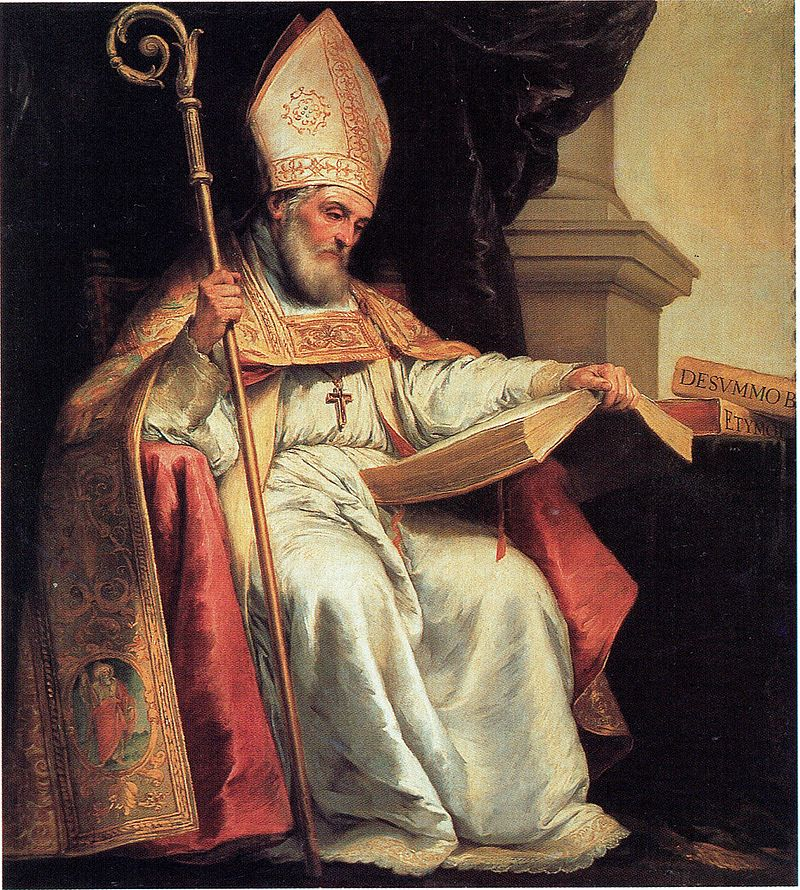
\includegraphics[scale=5.0]{isidorus.jpeg}

\thispagestyle{empty}

\pagebreak

\chapter{Western Romance}\label{cap:western_romance}

\epigraph{\textsc{venite igitvr descendamvs et confvndamvs ibi lingvam eorvm vt non avdiat vnvsqvisqve vocem proximi svi}}{\textsc{genesis} \textsc{xi}$\bullet$\textsc{vii}}

\section{Phonemic Inventory}

\subsection{Vocalic}

\begin{tcolorbox}[title=Western Romance Monophthongs, hbox]
  \begin{tabular}{|c|c|c|c|}
    \hline
    & Front & Central & Back \\
    \hline
    High & i & & u \\
    \hline
    Mid & e & & o \\
    \hline
    Low & & a & \\
    \hline
  \end{tabular}
\end{tcolorbox}

\subsection{Consonantal}

\begin{tcolorbox}[title=Western Romance Consonants, hbox]
  \begin{tabular}{|c|c|c|c|c|c|c|c|}
    \hline
    & Bilabial & Labiodental & Dental & Alveolar & Palatal & Velar & Labiovelar \\
    \hline
    Nasal & m & & \multicolumn{2}{c|}{n} & \textipa{\textltailn} & & \\
    \hline
    Stop & p \quad b & & t \quad d & & & k \quad g & \textipa{k\super w} \quad \textipa{g\super w} \\
    \hline
    Fricative & \textipa{B} & f & \textipa{D} & & & \textipa{G} & \\
    \hline
    \textquotedbl & & & & s \quad z & & & \\
    \hline
    Affricate & & & \textipa{\texttslig} \quad \textipa{\textdzlig} & & \textipa{\textteshlig} \quad \textipa{\textdyoghlig} & & \\
    \hline
    Trill & & & \multicolumn{2}{c|}{r} & & & \\
    \hline
    Lateral & & & \multicolumn{2}{c|}{l} & \textipa{L} & & \\
    \hline
  \end{tabular}
\end{tcolorbox}

\section{Sound Changes}

\subsection{Vocalism}

\subsubsection{Diphthongization I}\label{sec:diphthongization_1}

\begin{tcolorbox}

\end{tcolorbox}

\begin{tabular}{c c c}
  \textsc{lat.} & Es. & Fr. \\
  \hline
  \textsc{p\textcolor{red}{e}tra} & p\textcolor{magenta}{ie}dra & p\textcolor{magenta}{ie}rre \\
  \textsc{f\textcolor{red}{e}le} & h\textcolor{magenta}{ie}l & f\textcolor{magenta}{ie}l \\
  \textsc{v\textcolor{red}{e}nit} & v\textcolor{magenta}{ie}ne & v\textcolor{magenta}{ie}nt \\
  \textsc{h\textcolor{red}{e}ri} & a\textcolor{magenta}{ye}r & h\textcolor{magenta}{ie}r \\
\end{tabular}

\subsection{Consonantism}

\subsubsection*{Degemination}

\begin{tcolorbox}
  
\end{tcolorbox}

\begin{tabular}{c c}
  \textsc{lat.} & Es. \\
  \hline
  \textsc{o\textcolor{red}{ss}u} & hue\textcolor{magenta}{s}o \\
  \textsc{su\textcolor{red}{mm}a} & su\textcolor{magenta}{m}a \\
  \textsc{a\textcolor{red}{pp}e\textcolor{red}{ll}at} & a\textcolor{magenta}{p}e\textcolor{magenta}{l}a \\
  \textsc{li\textcolor{red}{tt}era} & le\textcolor{magenta}{t}ra \\
  \textsc{si\textcolor{red}{cc}u} & se\textcolor{magenta}{c}o \\
\end{tabular}

\subsubsection*{Lenition I}

\begin{tcolorbox}
  
\end{tcolorbox}

\begin{tabular}{c c}
  \textsc{lat.} & Es. \\
  \hline
  \textsc{sa\textcolor{red}{p}ore} & sa\textcolor{magenta}{b}or [\textipa{B}] \\
  \textsc{ca\textcolor{red}{p}ut} & ca\textcolor{magenta}{b}o [\textipa{B}] \\
  \textsc{co\textcolor{red}{p}ertu} & cu\textcolor{magenta}{b}ierto [\textipa{B}] \\
                & \\
  \textsc{vi\textcolor{red}{t}a} & vi\textcolor{magenta}{d}a [\textipa{D}] \\
  \textsc{fa\textcolor{red}{t}a} & ha\textcolor{magenta}{d}a [\textipa{D}] \\
  \textsc{ca\textcolor{red}{t}ena} & ca\textcolor{magenta}{d}ena [\textipa{D}] \\
                & \\
  \textsc{ami\textcolor{red}{c}a} & ami\textcolor{magenta}{g}a [\textipa{G}] \\
  \textsc{se\textcolor{red}{c}uru} & se\textcolor{magenta}{g}uro [\textipa{G}] \\
  \textsc{fo\textcolor{red}{c}u} & fue\textcolor{magenta}{g}o [\textipa{G}] \\
\end{tabular}

\begin{tabular}{c c}
  \textsc{lat} & Es. \\
  \hline
  \textsc{ca\textcolor{red}{b}allu} & ca\textcolor{magenta}{b}allo [\textipa{B}] \\
  \textsc{de\textcolor{red}{b}ere} & de\textcolor{magenta}{b}er [\textipa{B}] \\
  \textsc{ha\textcolor{red}{b}ere} & ha\textcolor{magenta}{b}er [\textipa{B}] \\
               & \\
  \textsc{cru\textcolor{red}{d}u} & cru\textcolor{magenta}{d}o [\textipa{D}] \\
  \textsc{pe\textcolor{red}{d}e} & pie \\
               & \\
  \textsc{au\textcolor{red}{g}ustu} & a\textcolor{magenta}{g}osto [\textipa{G}] \\
  \textsc{li\textcolor{red}{g}are} & li\textcolor{magenta}{g}ar [\textipa{G}] \\
  \textsc{pa\textcolor{red}{g}anu} & pa\textcolor{magenta}{g}ano [\textipa{G}] \\
\end{tabular}

\begin{tabular}{c c}  
  \textsc{lat.} & Es. \\
  \hline
  \textsc{le\textcolor{red}{p}re} & lie\textcolor{magenta}{b}re [\textipa{B}] \\
  \textsc{ca\textcolor{red}{p}ra} & ca\textcolor{magenta}{b}ra [\textipa{B}] \\
                & \\
  \textsc{pe\textcolor{red}{t}ra} & pie\textcolor{magenta}{d}ra [\textipa{D}] \\
  \textsc{pa\textcolor{red}{t}re} & pa\textcolor{magenta}{d}re [\textipa{D}] \\
                & \\
  \textsc{hemi-\textcolor{red}{c}rania} & mi\textcolor{magenta}{g}raña [\textipa{G}] \\
\end{tabular}

\begin{tabular}{c c}
  \textsc{lat.} & Es. \\
  \hline
  \textsc{ser\textcolor{red}{p}ente} & ser\textcolor{magenta}{p}iente \\
  \textsc{al\textcolor{red}{p}es} & a\textcolor{magenta}{p}les \\
  \textsc{rum\textcolor{red}{p}ere} & rum\textcolor{magenta}{p}er \\
                & \\
  \textsc{or\textcolor{red}{t}ica} & or\textcolor{magenta}{t}iga \\
  \textsc{men\textcolor{red}{t}a} & men\textcolor{magenta}{t}a \\
                & \\
  \textsc{ar\textcolor{red}{c}u} & ar\textcolor{magenta}{c}o \\
  \textsc{fal\textcolor{red}{c}one} & hal\textcolor{magenta}{c}ón \\
\end{tabular}

The orthography of Visigothic texts shows signs of lenition and the confusion was caused by it \parencite[p.~159]{latin_palaeography}:
\begin{quote}
  The use of \emph{b} instead of \emph{p} (\emph{abtum}) or \emph{p} for \emph{b} (\emph{puplicum}), \emph{g} for \emph{c} (\emph{eglesia}\footnote{cf. Es. \emph{iglesia}}) or the reverse (\emph{intecritate}), \emph{k} for \emph{c} (\emph{kaput}), \emph{t} for \emph{d} (\emph{aput}) or \emph{d} for \emph{t} (\emph{sustinead}).
\end{quote}

\pagebreak

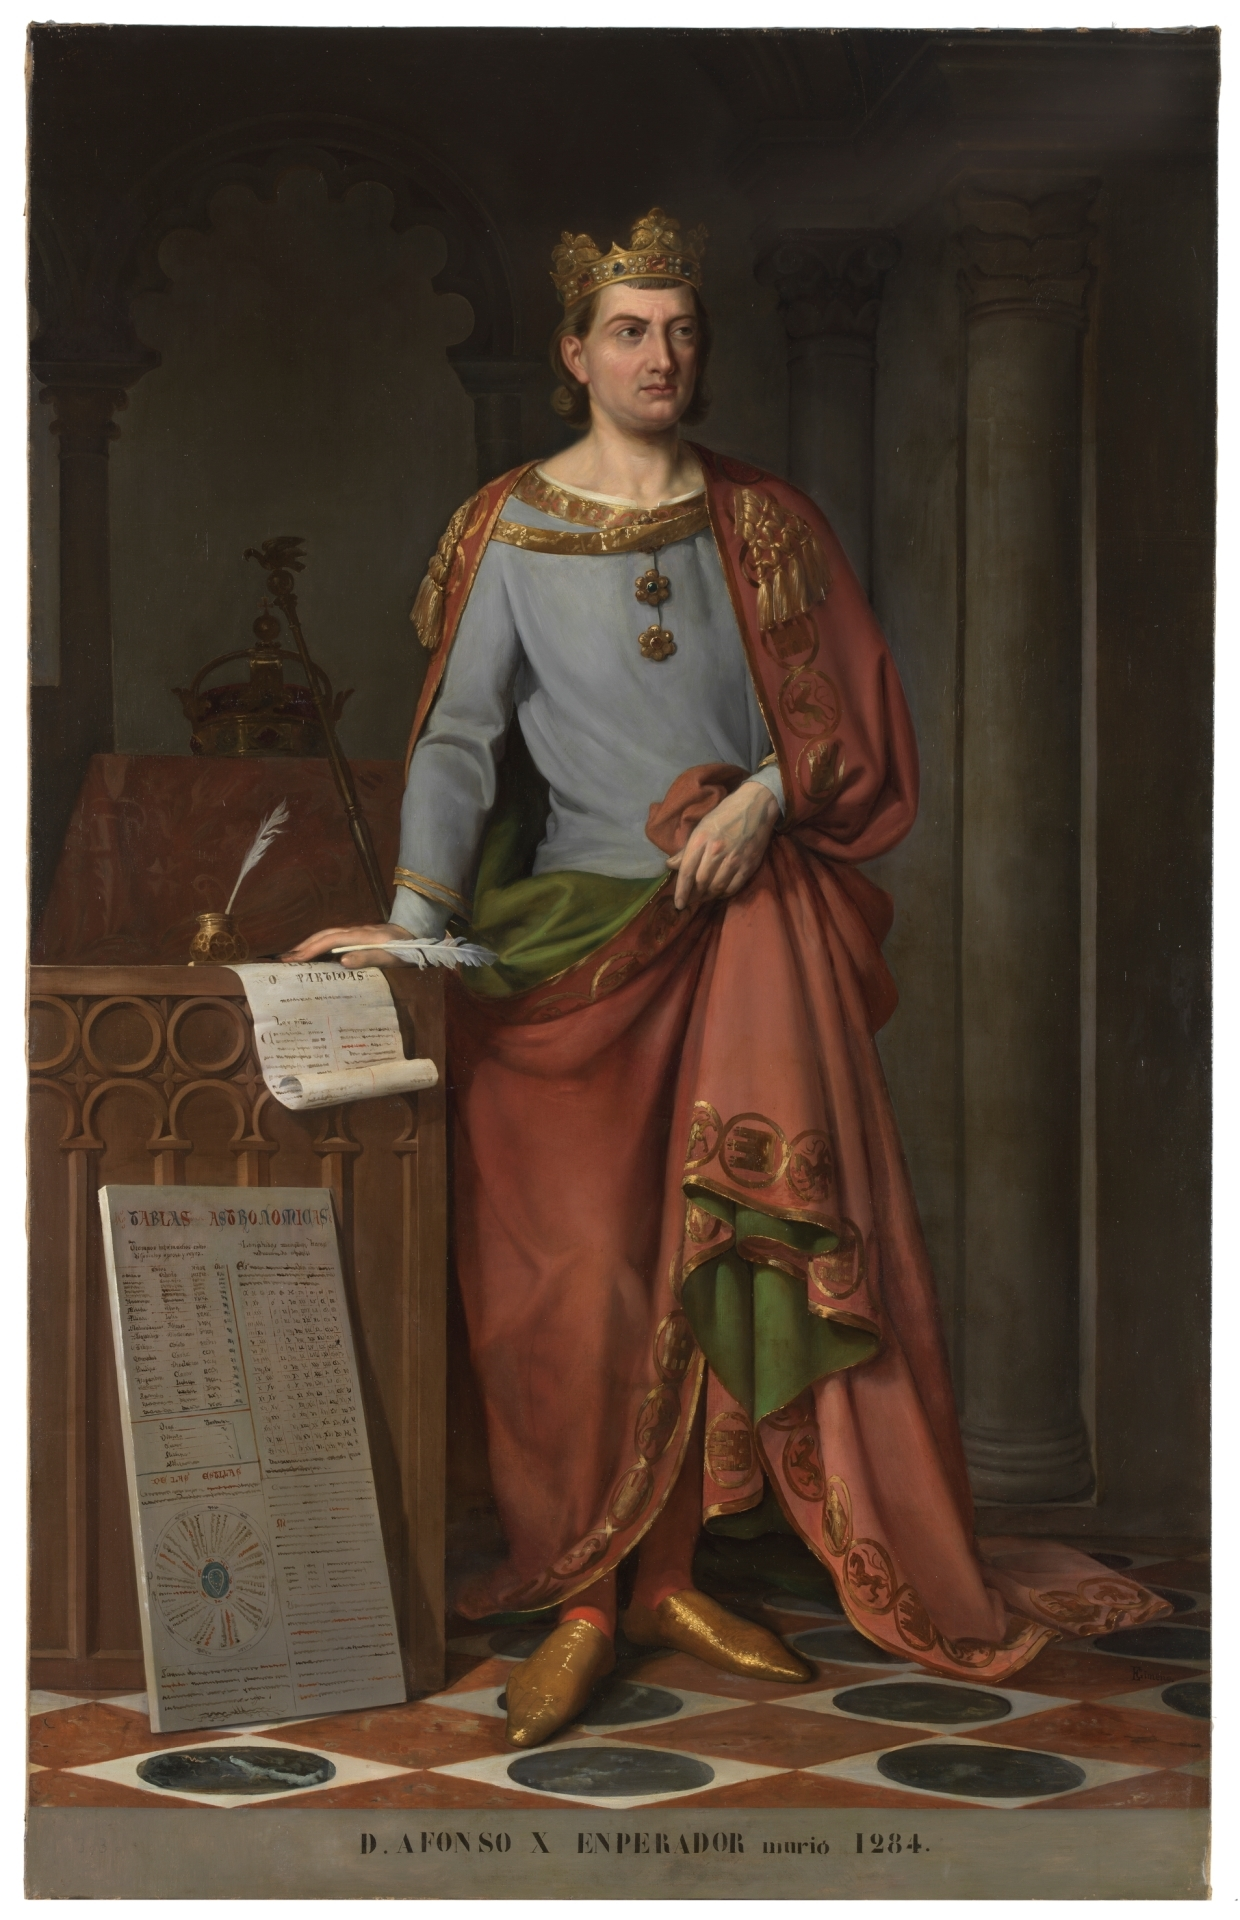
\includegraphics[scale=0.45]{alfonso_x.jpg}

\thispagestyle{empty}

\pagebreak

\chapter{Old Spanish}

\epigraph{Ya lo vedes, que partirnos emos en vida, yo iré e vós fincaredes remanida.}{Cantar de Mio Cid}

\section{Phonemic Inventory}

\subsection{Vocalic}

\begin{tcolorbox}[title=Old Spanish Monophthongs, hbox]
  \begin{tabular}{|c|c|c|c|}
    \hline
    & Front & Central & Back \\
    \hline
    High & i & & u \\
    \hline
    Mid & e & & o \\
    \hline
    Low & & a & \\
    \hline
  \end{tabular}
\end{tcolorbox}

\subsection{Consonantal}

\begin{tcolorbox}[title=Old Spanish Consonants, hbox]
  \begin{tabular}{|c|c|c|c|c|c|c|c|c|}
    \hline
    & Bilabial & Labiodental & Dental & Alveolar & Palatal & Velar & Labiovelar & Glottal \\
    \hline
    Nasal & m & & \multicolumn{2}{c|}{n} & \textipa{\textltailn} & & & \\
    \hline
    Stop & p \quad b & & t \quad d & & & k \quad g & \textipa{k\super w} \quad \textipa{g\super w} & \\
    \hline
    Fricative & \textipa{F} \quad \textipa{B} & f & \textipa{D} & & \textipa{J} & \textipa{G} & & h \\
    \hline
    \textquotedbl & & & & s \quad z & \textipa{S} \quad \textipa{Z} & & & \\
    \hline
    Affricate & & & \textipa{\texttslig} \quad \textipa{\textdzlig} & & \textipa{\textteshlig} \quad \textipa{\textdyoghlig} & & & \\
    \hline
    Trill & & & \multicolumn{2}{c|}{r} & & & & \\
    \hline
    Tap & & & \multicolumn{2}{c|}{\textipa{R}} & & & & \\
    \hline
    Lateral & & & \multicolumn{2}{c|}{l} & \textipa{L} & & & \\
    \hline
  \end{tabular}
\end{tcolorbox}

\section{Sound Changes}

\subsection{Vocalism}

\subsubsection{Diphthongization II}\label{sec:diphthongization_2}

\begin{tcolorbox}
  
\end{tcolorbox}

\begin{tabular}{c c}
  \textsc{lat.} & Es. \\
  \textsc{hib\textcolor{red}{e}rnu} & inv\textcolor{magenta}{ie}rno \\
  \textsc{ap\textcolor{red}{e}rta} & ab\textcolor{magenta}{ie}rta \\
  \textsc{s\textcolor{red}{e}pte} & s\textcolor{magenta}{ie}te \\
  \textsc{c\textcolor{red}{e}rvu} & c\textcolor{magenta}{ie}rvo \\
  \textsc{f\textcolor{red}{e}rru} & h\textcolor{magenta}{ie}rro \\
  \textsc{f\textcolor{red}{o}rte} & f\textcolor{magenta}{ue}rte \\
  \textsc{p\textcolor{red}{o}rta} & p\textcolor{magenta}{ue}rta \\
  \textsc{m\textcolor{red}{o}rdit} & m\textcolor{magenta}{ue}rde \\
  \textsc{m\textcolor{red}{o}rit} & m\textcolor{magenta}{ue}re \\
  \textsc{m\textcolor{red}{o}vet} & m\textcolor{magenta}{ue}ve \\
  \textsc{p\textcolor{red}{o}tet} & p\textcolor{magenta}{ue}de \\
\end{tabular}

\subsubsection*{Metaphony}

\begin{tcolorbox}
  
\end{tcolorbox}

\begin{tabular}{c c}
  \textsc{lat.} & Es. \\
  \hline
  \textsc{m\textcolor{red}{u}ltu} & m\textcolor{magenta}{u}cho \\
  \textsc{ausc\textcolor{red}{u}ltat} & esc\textcolor{magenta}{u}cha \\
  \textsc{l\textcolor{red}{a}cte} & l\textcolor{magenta}{u}cha \\
  \textsc{l\textcolor{red}{a}cte} & l\textcolor{magenta}{e}che \\
  \textsc{f\textcolor{red}{a}ctu} & h\textcolor{magenta}{e}cho \\
  \textsc{b\textcolor{red}{a}siu} & b\textcolor{magenta}{e}so \\
  \textsc{c\textcolor{red}{a}seu} & q\textcolor{magenta}{ue}so \\
  \textsc{r\textcolor{red}{e}ni\={o}ne} & r\textcolor{magenta}{i}ñón \\
  \textsc{g\textcolor{red}{e}nesta} & h\textcolor{magenta}{i}niesta \\
  \textsc{c\textcolor{red}{ae}mentum} & c\textcolor{magenta}{i}miento \\
  \textsc{t\textcolor{red}{e}nebras} & t\textcolor{magenta}{i}nieblas \\
  \textsc{c\textcolor{red}{o}chle\={a}re} & c\textcolor{magenta}{u}chara \\
  \textsc{c\textcolor{red}{o}gn\={a}tu} & c\textcolor{magenta}{u}ñado \\
  \textsc{m\textcolor{red}{u}liere} & m\textcolor{magenta}ujer \\
\end{tabular}

\subsubsection*{Reduction of Final Vowels}

\begin{tcolorbox}

\end{tcolorbox}

\begin{tabular}{c c}
  \textsc{lat.} & Es. \\
  \hline
  \textsc{v\={e}n\={i}} & vine \\  
\end{tabular}

\begin{tabular}{c c}
  OSp. & Es. \\
  \hline
  m\textcolor{red}{ía} & (*m\textcolor{red}{íe} $\rightarrow$) m\textcolor{magenta}{i} \\
  du\textcolor{red}{a}s & du\textcolor{magenta}{e}s \\
  primer\textcolor{red}{o} & primer \\
  tercer\textcolor{red}{o} & tercer \\
  sant\textcolor{red}{o} & san \\
  segund\textcolor{red}{o} & según \\
\end{tabular}

\begin{tabular}{c c}
  \textsc{lat.} & Es. \\
  \hline
  \textsc{pariet\textcolor{red}{e}} & pared \\
  \textsc{merced\textcolor{red}{e}} & merced \\
  \textsc{p\={a}n\textcolor{red}{e}} & pan \\
  \textsc{mar\textcolor{red}{e}} & mar \\
  \textsc{fid\={e}l\textcolor{red}{e}} & fiel \\
  \textsc{p\={a}c\textcolor{red}{e}} & paz \\
  \textsc{calc\textcolor{red}{e}} & coz \\
  \textsc{falc\textcolor{red}{e}} & hoz \\
  \textsc{fasc\textcolor{red}{e}} & haz \\
  \textsc{pisc\textcolor{red}{e}} & pez \\
\end{tabular}

\subsection{Consonantism}

\subsubsection*{Palatalization of Clusters}

\begin{tcolorbox}

\end{tcolorbox}

\begin{tabular}{c c}
  \textsc{lat.} & Es. \\
  \hline
  \textsc{di\textcolor{red}{ct}u} & di\textcolor{magenta}{ch}o [\textipa{\textteshlig}] \\
  \textsc{stri\textcolor{red}{ct}u} & estre\textcolor{magenta}{ch}o [\textipa{\textteshlig}] \\
  \textsc{pe\textcolor{red}{ct}u} & pe\textcolor{magenta}{ch}o [\textipa{\textteshlig}] \\
  \textsc{te\textcolor{red}{ct}u} & te\textcolor{magenta}{ch}o [\textipa{\textteshlig}] \\
  \textsc{no\textcolor{red}{ct}e} & no\textcolor{magenta}{ch}e [\textipa{\textteshlig}] \\
  \textsc{o\textcolor{red}{ct}o} & o\textcolor{magenta}{ch}o [\textipa{\textteshlig}] \\
\end{tabular}

\subsubsection*{Metathesis}

\begin{tcolorbox}

\end{tcolorbox}

\subsubsection*{Debuccalization of /f/}

\begin{tcolorbox}
  
\end{tcolorbox}

\begin{tabular}{c c}
  \textsc{lat.} & Es. \\
  \hline
  \textsc{\textcolor{red}{f}ilu} & \textcolor{magenta}{h}ilo \\
  \textsc{\textcolor{red}{f}erire} & \textcolor{magenta}{h}erir \\
  \textsc{\textcolor{red}{f}erro} & \textcolor{magenta}{h}ierro \\
  \textsc{\textcolor{red}{f}alcone} & \textcolor{magenta}{h}alcón \\
                & \\
  \textsc{\textcolor{red}{f}ocu} & \textcolor{magenta}{f}uego \\
  \textsc{\textcolor{red}{f}ora} & \textcolor{magenta}{f}uera \\
  \textsc{\textcolor{red}{f}onte} & \textcolor{magenta}{f}uente \\
  \textsc{\textcolor{red}{f}ronte} & \textcolor{magenta}{f}rente \\
  \textsc{\textcolor{red}{f}lore} & \textcolor{magenta}{f}lor \\
  \textsc{\textcolor{red}{f}laccu} & \textcolor{magenta}{f}laco \\
\end{tabular}

\pagebreak

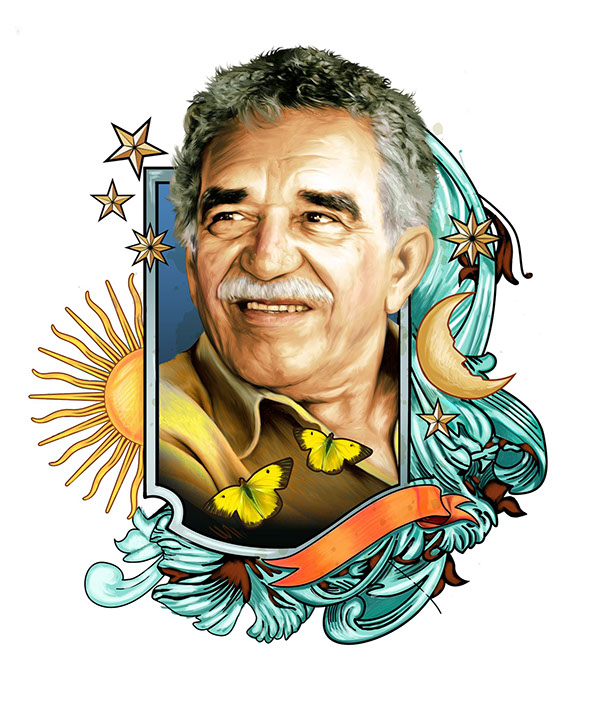
\includegraphics[scale=0.75]{marquez.jpg}

\thispagestyle{empty}

\pagebreak

\chapter{Modern Spanish}

\epigraph{Todo está cumplido.}{Juan 19:30}

\section{Phonemic Inventory}

\subsection{Vocalic}

\subsection{Consonantal}

\section{Sound Changes}

\subsection{Vocalism}

\subsection{Consonantism}

\subsubsection*{Lenition II}

\begin{tcolorbox}

\end{tcolorbox}

\subsubsection*{Betacism II}

\begin{tcolorbox}

\end{tcolorbox}

\subsubsection*{Simplication of Clusters}

\begin{tcolorbox}
  
\end{tcolorbox}

\subsubsection*{Deaffrication}

\begin{tcolorbox}

\end{tcolorbox}

\subsubsection*{Devoicing of Fricatives}

\begin{tcolorbox}
  
\end{tcolorbox}

\subsubsection*{The Fate of Dental Affricates}

\begin{tcolorbox}

\end{tcolorbox}

\subsubsection*{Retraction of Palatal Fricative}

\begin{tcolorbox}
  
\end{tcolorbox}

\chapter{Anthology of Sound Changes}

\section{\emph{Zen} and Sound Changes}

\subsection{Syllabificaiton and Serialization}

\subsection{Phonotactics and Repairment}

\subsection{Phonological Word: Maybe not So Flat of a Structure}

\chapter{Sunday School with the Wug}

The linguistic history part of this paper is over; but Spanish and her predecessors are so rich in morpho-syntax. It would be a shame to write a paper on Spanish without having a single paper dedicated to its morpho-syntactic aspect, hence we compensate by having a small chapter dedicated to a couple verses in the \emph{Gospel of John} and a couple \emph{sayings on the cross}, comparing the scripture in Latin, Old Spanish, and Modern Spanish. \\
The Latin verses are from \textsc{Nova Vulgata}, the Old Spanish verses from \emph{Evangelios y Epístolas paulinas de Mart\'{i}n de Lucena} \footcite{osp_nt} (the text presented here is normalized by me), and Modern Spanish ones from \emph{La Biblia de Jerusal\'{e}n}. The English glosses and exegetic notes are taken from the beloved \emph{Oxford Annotated Bible}\footcite{oab}, based on the \emph{New Revised Standard Version} translation. Since we are dealing with the Bible in many languages, the abbreviation of the Gospels will be in Latin, \textsc{e.g.} \textsc{Ioannes}, instead of \emph{Juan} or \emph{John}.

\section{Ioannes 1:1--5}

\begin{tcolorbox}[title=\textsc{Nova Vulgata}]
  \textsc{$^1$ in principio erat verbum et verbum era tapud deum et deus erat verbum} \\
  \textsc{$^2$ hoc erat in principio apud deum} \\
  \textsc{$^3$ omnia per ipsum facta sunt et sine ipso factum est nihil quod factum est} \\
  \textsc{$^4$ in ipso vita erat et vita erat lux hominum} \\
  \textsc{$^5$ et lux in tenebris lucet et tenebrae eam non comprehenderunt} \\
\end{tcolorbox}

\begin{tcolorbox}[title=Evangelios y Epístolas paulinas de Mart\'{i}n de Lucena]
  $^1$ Enel comien\c{c}o era palabra e la palabra era \c{c}erca de dios e dios era palabra \\
  $^2$ aquesto era en prin\c{c}ipio \c{c}erca de dios \\
  $^3$ todas las cosas por el son fechas e syn el non es fecha alguna cosa lo que fue fecho \\
  $^4$ enel vida era e la vida era luz delos ombres \\
  $^5$ e la luz enlas tiniebras luze e las tiniebras non la comprehendieron \\
\end{tcolorbox}

\begin{tcolorbox}[title=La Biblia de Jerusal\'{e}n]
  $^1$ En el principio exist\'{i}a la Palabra y la Palabra estaba con Dios, y la Palabra era Dios. \\
  $^2$ Ella estaba en el principio con Dios. \\
  $^3$ Todo se hizo por ella y sin ella no se hizo nada de cuanto existe. \\
  $^4$ En ella estaba la vida y la vida ear la luz de los hombres, \\
  $^5$ y la luz brilla en las tinieblas, y las tinieblas no la vencieron. \\
\end{tcolorbox}

\subsection{Ioannes 1:1}

\begin{exe}
  \sn
  \glll 
  \textsc{in} \textsc{principio} \textsc{erat} \textsc{verbum} \\
  enel comien\c{c}o era palabra \\
  {En el} principio exist\'{i}a {la Palabra} \\
  \glt 
  ``In the beginning was the Word[.]''
\end{exe}

\begin{exe}
  \sn
  \glll
  \textsc{et} \textsc{verbum} \textsc{erat} \textsc{apud} \textsc{deum} \\
  e {la palabra} era {\c{c}erca de} dios \\
  y {la Palabra} estaba con Dios \\
  \glt
  ``[A]nd the Word was with God[.]''
\end{exe}

\begin{exe}
  \sn
  \gll
  \textsc{et} \textsc{deus} \textsc{erat} \textsc{verbum}\\
  e dios era palabra \\
  \glt
  ``[A]nd the Word was God.''
\end{exe}

\begin{exe}
  \sn
  \gll
  y la Palabra era Dios. \\
  and the Word was God. \\
\end{exe}

\subsection{Ioannes 1:2}

\begin{exe}
  \sn
  \glll
  \textsc{hoc} \textsc{erat} \textsc{in} \textsc{principio} \textsc{apud} \textsc{deum} \\
  aquesto era en prin\c{c}ipio {\c{c}erca de} dios \\
  Ella estaba {en el} principio con Dios \\
  \glt
  ``He was in the beginning with God.''
\end{exe}

\subsection{Ioannes 1:3}

\subsection{Ioannes 1:4}

\subsection{Ioannes 1:5}

\section{\emph{Saysing on the Cross}}

\subsection{\emph{Today shalt thou be with me in paradise.}}

\subsection{\emph{My God, my God, why hast thou forsaken me?}}

\subsection{\emph{It is finished.}}

\chapter{Epilogue: Mein liebster Jugendtraum}

\epigraph{I have fought the good fight; \\ I have finished the race; \\ I have kept the faith.}{2 Timothy 4:7}

Other than the historical phonology of Latin and Spanish, there is yet another \emph{Jugendtraum} of mine: that is the historical phonology of the Sinitic languages.

\section{Die Rekonstruktion der Altchinesische}

\subsection{Phonemic Inventory}

\subsection{Syllabic Structure}

\subsection{Sound Changes to Middle Chinese}

\subsubsection{Vocalism}

\subsubsection{Consonantism}

\subsubsection{Tonogenesis}

\section{\emph{THE BOOK} of Sound Laws}

\epigraph{Prove and conjecture and keep the SF's score low.\footnotemark}{Erd\H{o}s P\'{a}l}
\footnotetext{\href{https://www.youtube.com/watch?v=AW97QTNf5ig}{The Purpose of Life.}}

Erd\H{o}s P\'{a}l talks about ``The Book, in which God maintains the perfect proofs for mathematical theorems, following the dictum of G. H. Hardy that there is no permanent place for ugly mathematics'' \parencite[p.~5]{proofs_from_the_book}. I, too, think that there exists a \emph{Book} of sound laws that can be formalized computationally in a beautiful computer language (it has to be \emph{beautiful}, in the same spirit of Hardy's words, very little place is reserved for ugly linguistics). And this, dare I say, \emph{program} is what I want dedicate the next few years of my life to. \\

\nocite{*}

\chapter*{Bibliography}
\addcontentsline{toc}{chapter}{Biblipgraphy}

\printbibliography[heading=subbibintoc, keyword=phone, title={Phonology}]

\printbibliography[heading=subbibintoc, keyword=romance, title={Romance Linguistics}]

\printbibliography[heading=subbibintoc, keyword=tcs, title={Computation}]

\printbibliography[heading=subbibintoc, keyword=misc, title = {Misc.}]

\end{document}
